% #############################################################################
% This is Chapter 2
% !TEX root = ../main.tex
% #############################################################################
% Change the Name of the Chapter i the following line
\fancychapter{Background and Related Work}
\cleardoublepage
% The following line allows to ref this chapter
\label{chap:background}

This chapter details the technical concepts required to understand the problem, the proposed solution and the rationale behind it. It starts by providing an overview of cryptographic services, primitives and protocols. Then, it presents several general purpose computing systems which offer cryptographic services, and ends by presenting other relevant components.

%%%%%%%%%%%%%%%%%%%%%%%%%%%%%%%%%%%%%%
\section{Cryptography and Other Concepts}\label{chap:background:crypto}

There are four important cryptographic services relevant for this work. Confidentiality is used to scramble information and hide the content from unauthorized entities. Integrity protects data from unauthorized modification. Authentication ascertains the origin of a message. Non-Repudiation prevents an entity from denying the authorship of a document or message.
To guarantee these services, two types of key infrastructure exist: symmetric and asymmetric. 
Symmetric keys are shared by two or more communicating parties. The same key is used to encrypt and decrypt data, or for other services. The keys are generally smaller and the operations faster than with asymmetric keys. Asymmetric keys constitute a pair for each side, a private and a public key. The private key is personal and should never be shared. The public key may be shared widely.

There are two types of ciphers: stream and block ciphers. Stream ciphers usually process 1 bit of data at a time. Stream ciphers are usually faster than block ciphers, have lower memory requirements and thus are more suitable to embedded devices with limited memory. Block ciphers encrypt fixed-length groups of bits, called blocks. They have a higher memory usage, in order to keep the blocks in memory. The processed data needs to be padded to a multiple of the block size. This can introduce problems if not done correctly. Another caveat of block ciphers is they are more susceptible to noise in transmissions. If a bit is flipped in a stream cipher, only the corresponding bit is affected, while with a block cipher, more than 1 bit can be affected.

%%%%%%%%%%%%%%%%%%%%%%%%%%%%%%%%%%%%%%
\subsection{Hash Functions}\label{chap:background:crypto:hash}

A cryptography hash function generates a fixed dimension value (digest) based on input texts, such as messages or files. Secure hashes provide message integrity by comparing digests, calculated before and after transmission, to determine if the message was modified. The same message always generates the same digest.
To achieve this, hash functions must have several properties. The same input value always results in the same hash. Very different outputs must be generated from very similar inputs. It should be hard to find two messages which generate the same hash and it should be hard to find an input that produces a given hash.
Popular and recommended hash functions include \ac{SHA}-2 and the newer \ac{SHA}-3~\cite{dang2015secure}. Both versions have variants. For example, the \ac{SHA}-256 function produces a 256 bit digest and \ac{SHA}-512 a 512 bit digest.
% \begin{enumerate}
%     \item They must be deterministic, meaning the same input value must always result in the same hash value;
%     \item They must generate very different output values for similar inputs;
%     \item They must be collision resistant, meaning it should be hard to find two input messages that generate the same hash value;
%     \item The hash value should be computed relatively quickly;
%     \item Given a hash value, it should be hard to find an input text that produces that hash value.
% \end{enumerate}

%%%%%%%%%%%%%%%%%%%%%%%%%%%%%%%%%%%%%%
\subsection{Symmetric Encryption}\label{chap:background:crypto:symmetric}

Symmetric ciphers are frequently used to provide authentication and confidentiality, using symmetric keys.
\ac{AES} is one of the most popular symmetric-key algorithms. It has multiple block and stream cipher modes, which offer confidentiality. It uses 128-bit blocks and keys can have 128, 192 or 256 bits. Some relevant AES encryption modes are presented next.

\textbf{\ac{ECB}} is the simplest mode. It is a block cipher and works by encrypting each block with the symmetric key. If the same key is used for equal plaintext blocks, the result will always be the same. For this reason, patterns are easily seen and the mode is considered insecure.

\textbf{\ac{CBC}} is another block cipher mode. It combines the first block of plaintext and an \ac{IV} with the XOR operator and encrypts the result. For the subsequent blocks, the previous ciphertext is used instead of the IV. The message needs to be padded to a multiple of the block size. If done incorrectly, the mode is vulnerable to padding oracle attacks \cite{paddingoracle}. Implementing ciphertext stealing, which avoids padding, is recommended for the security of \ac{CBC} \cite{ciphertextstealing}.

\textbf{\ac{OFB}} mode repeatedly encrypts the IV for each block, xoring the result with the plaintext block. The encryption and decryption processes are exactly the same.
The block cipher is only used in the encryption direction, which means the message does not need to be padded. Therefore, it is a stream cipher.

\textbf{\ac{CTR}} mode concatenates an IV with a counter beginning at 0. This sequence is encrypted and applied to the xor operation with the plaintext block. For each block the sequence is incremented by 1.
This mode is comparable to \ac{OFB}, as it is also a stream cipher and the encryption operation is exactly the same as the decryption. 

The \ac{IV} needs to be sent along with the ciphertext to the receiver, or the receiver will not be able to retrieve the entire message. There is no need for the IV to be kept secret.
\ac{CBC}, \ac{OFB} and \ac{CTR} modes are proved secure, assuming the \ac{IV} is random and unique, meaning it is only used once for each key and message.
Regarding performance, \cite{aesmodes} states \ac{CBC} is slower than \ac{CTR} mode, and \ac{OFB} is even slower.
When efficiency characteristics matter, nothing comes close to \ac{CTR}: it has better performance characteristics, compared to \ac{CBC} and \ac{OFB}.

All these cipher modes are malleable, meaning an attacker can modify a ciphertext C, to create ciphertext C' which will decrypt to plaintext P' that is similar to the original plaintext. Malleability is connected to message integrity. This is not considered a relevant weakness since these modes are only designed to offer confidentiality. If integrity is needed, one of these modes should be paired with a \ac{MAC}, or instead use a dedicated authenticated-encryption mode like \ac{CCM} or \ac{GCM} (discussed in Section~\ref{chap:background:crypto:aead}), which guarantee both confidentiality and integrity.

%%%%%%%%%%%%%%%%%%%%%%%%%%%%%%%%%%%%%%
\subsection{Message Authentication Code}\label{chap:background:crypto:mac}

\ac{MAC} is a value, also called tag, used for authenticating a message.
A \ac{MAC} algorithm generates a tag from a message and symmetric key. Unlike digital signatures, \ac{MAC} does not offer non-repudiation since it uses a symmetric key, which is shared among all users. Anyone in possession of the key can generate a \ac{MAC} for a message, as well as, verify a MAC generated with the same key. On the contrary, digital signatures utilize the private key of an asymmetric pair to generate, and public key to verify.
Several techniques exist to construct a \ac{MAC}. One is \textbf{\ac{CBC-MAC}}, which utilizes the \ac{CBC} block cipher to encrypt data. A chain of blocks is generated, and the last block is the tag.
\ac{CBC-MAC} also has similar caveats to \ac{CBC}, it is only secure for fixed-length messages \cite{aesmodes} and different keys have to be used for \ac{CBC} encryption and tag generation.

\textbf{\ac{HMAC}} is different, it uses a cryptographic hash function, such as SHA-2, and a symmetric secret key to construct a tag. \ac{HMAC} is secure, as long as the underlying hash function used is secure. Therefore SHA-2 is a good option.
\ac{HMAC} does not have the security problems of \ac{CBC-MAC}. It is a popular and well-designed construction, but it is not the most efficient approach~\cite{aesmodes}.
% \ac{CBC-MAC} security deficiencies were resolved with \ac{OMAC}, which is secure for variable-length messages.
%Despite \ac{CBC}'s inefficiencies, \ac{HMAC} is slower due to the hashing operations.

%%%%%%%%%%%%%%%%%%%%%%%%%%%%%%%%%%%%%%
\subsection{Authenticated Encryption}\label{chap:background:crypto:aead}

\ac{AEAD} schemes assure confidentiality and authenticity using symmetric keys. They may be more efficient than combining separate encryption and authentication techniques, such as the ones discussed in earlier sections, and are less likely to be used incorrectly. \ac{AEAD} schemes also allow associated data to be included in the message, which is authenticated but not encrypted. This feature is useful for network packets. The header is visible but is authenticated, while the payload is encrypted and authenticated. 
\ac{AES} has several of these schemes. 

\textbf{\ac{CCM}} is an \ac{AEAD} mode that combines \ac{CBC-MAC} for authentication with \ac{CTR} for confidentiality.
\ac{CCM} uses a MAC-then-Encrypt approach. First, the \ac{MAC} is computed from the message. Then the message and the tag are encrypted with \ac{CTR} mode.
Due to performing two encryption operations, \ac{CBC-MAC} and then \ac{CTR}, the mode is not as efficient compared to others such as \ac{GCM}, which only performs one encryption operation.
It is not an online mode, meaning it needs to know the message and \ac{AD} length beforehand. Therefore, \ac{AD} cannot be preprocessed. 
Despite being a slower mode, it is secure and widely supported. It is included in \ac{IPsec}, \ac{TLS} and Bluetooth low energy.

\textbf{\ac{GCM}} utilizes an encrypt-then-MAC approach. It first encrypts with \ac{CTR} mode, then uses Galois mode of authentication to generate the tag. The Galois field multiplication supports parallel computation, making this mode faster than \ac{CCM}.
Beyond being parallelizable, it is online and the \ac{AD} can be preprocessed.
For security reasons, authentication tags should be at least 96 bits, even though the mode allows smaller tags. One limitation of \ac{GCM} is, it can encrypt a maximum of 64 gigabytes of plaintext. Security analysis of several modes decisively states that \ac{GCM} in hardware is unsurpassed by any authenticated-encryption scheme~\cite{aesmodes}.

%%%%%%%%%%%%%%%%%%%%%%%%%%%%%%%%%%%%%%
\subsection{Asymmetric Encryption}\label{chap:background:crypto:assymetric}

Asymmetric cryptography uses public and private keys. It is commonly used to provide confidentiality, data integrity, authentication and non-repudiation.
The private key must always remain secure with the owner. Public keys may be distributed. Encrypting a message with the public key provides confidentiality, since only the owner who possesses the private key can decipher the message. On the other hand, private key encryption provides authentication, since only the owner is in possession of the private key. These two different concepts can be combined to provide confidentiality, authentication and non-repudiation to a message, through digital signatures.

Compared to symmetric keys, asymmetric keys are less risky to distribute, as the public key can be viewed by anyone. However, there is the problem of validating public keys, which consists of guaranteeing a public key is owned by the correct identity.
Once two parties have traded public keys, asymmetric and symmetric keys can be combined in a hybrid encryption scheme. It takes advantage of the faster symmetric encryption to cipher the data, and the asymmetric encryption to encrypt the symmetric key, and provide authentication. Alternatively, it can be used to share symmetric keys for usage with an authenticated-encryption scheme.

There are two popular algorithms for public-key encryption, \ac{RSA} and \ac{ECC}~\cite{mahto2016security}.
\ac{RSA} has been used for decades, is well established and widely used. It is based on the difficulty of factoring the product of two large prime numbers.
\ac{ECC} is a more recent algorithm, based on the Elliptic Curve Discrete Logarithm Problem. The main advantage of \ac{ECC} is it offers the same level of security, with a smaller key size. According to Gupta \& Silakari, 2011~\cite{eccoverrsa}, a 160-bit \ac{ECC} private key has similar security to a 1024-bit \ac{RSA} key.
\ac{ECC} operations are potentially faster with smaller key sizes, so this makes elliptic curve based schemes more suited for less powerful and memory constrained devices \cite{selvakumaraswamy2016efficient}.
With the threat of quantum computers, both \ac{ECC} and \ac{RSA} could become obsolete in the future, as they are vulnerable to brute force attacks from such devices.
% useful for small wireless devices with processing power, storage space, or power consumption restrictions.
%They also state that smaller key sizes may result in faster execution timings for the schemes, which is beneficial to systems where real time performance is a critical factor.

%%%%%%%%%%%%%%%%%%%%%%%%%%%%%%%%%%%%%%
\subsection{Diffie-Hellman}\label{chap:background:crypto:ecdh}

The \ac{DH} key exchange algorithm allows two parties to agree on a shared secret, which can be used to derive a symmetric key. Both parties compute the secret from publicly exchanged integers, and private integers. Attackers listening on the exchanged public integers cannot compute the same secret, since both sides' private integers are never shared.

\ac{ECDH} key exchange is similar, it computes the shared secret from \ac{ECC} private and public keys, instead of integers. Incorporating \ac{ECC} keys provides the same level of security compared with integers, but with a smaller bit size ~\cite{fiskiran2002workload}.

%%%%%%%%%%%%%%%%%%%%%%%%%%%%%%%%%%%%%%
\subsection{Digital Signatures}\label{chap:background:crypto:signatures}

Signatures are a standard scheme for authenticating digital messages and ensuring the signer cannot repudiate the signature. A digital signature is generated by combining asymmetric cryptography and a hash function.
A digital signature is generated by first computing a hash of the message, then signing the hash with the author's private key. The message is not directly signed, since public-key encryption is slow and messages are most likely bigger than the hash of a message, which has a fixed size. Third parties can validate the signature using the author's public key. Only the author, in possession of their private key, could have generated the signature.
Digital signatures are a digital version of handwritten signatures~\cite{digitalsignatures}, commonly used anywhere forgery detection is essential, for instance in financial transactions or software distribution.
A popular digital signatures algorithm with ECC keys is \ac{ECDSA}.

Qualified signatures are a special type of signatures where the private keys are generated and stored inside a device, such as a Smart Card, and are never exposed to the outside. For the owner to sign a document, the Smart Card is needed (something owned) and a \ac{PIN} (something known). This strong signature legally represents a person or a group. This type of signatures are used in the Portuguese Citizen Card.

%%%%%%%%%%%%%%%%%%%%%%%%%%%%%%%%%%%%%%
\subsection{Transport Layer Security}\label{chap:background:TLS}

\ac{TLS} is a cryptographic protocol that aims to provide confidentiality and data integrity, during transmission, over the \ac{TCP}. It uses symmetric cryptography to encrypt data. A new set of symmetric keys is generated for each connection.
TLS supports asymmetric cryptography which authenticates the identity of the communicating parties.
TLS is widely used in web browsing, e-mail and instant messaging.
The protocol can provide perfect forward secrecy, assuring any past connections are secure, if in the future encryption keys are compromised.

%%%%%%%%%%%%%%%%%%%%%%%%%%%%%%%%%%%%%%
\subsection{Public Key Infrastructure}\label{chap:background:PKI}

Asymmetric cryptography needs a secure mechanism to validate public keys, achieved by guaranteeing a public key is owned by a certain identity.
A \ac{PKI} is a central database of public-key certificates. It is responsible for managing, distributing, storing and revoking digital certificates. Digital certificates map public keys to identities, and are used to verify that a specific public key belongs to a given identity.
A \ac{PKI} has several components, e.g., a registration authority, a certification authority and a central database of stored keys.
A user can submit other entities' public keys. Entities that trust the user responsible for the submission can use the public keys.
There are alternative approaches to \ac{PKI}, such as a web of trust. This mechanism uses self-signed certificates and third parties attest these certificates. This approach is implemented in \ac{PGP}~\cite{modelingPKI}.

%%%%%%%%%%%%%%%%%%%%%%%%%%%%%%%%%%%%%%
\subsection{Random Number Generators}

A \ac{TRNG} can generate a sequence of numbers that cannot be predicted. Generating random numbers is a common and critical requirement for most cryptographic algorithms. Pseudo-random number generators are frequent in software approaches and are not truly random. They depend on an algorithm and initial conditions (seed) to generate random numbers. If the seed is known, the numbers are predictable.
\ac{TRNG} are hardware devices that generate numbers from unpredictable physical conditions. For this reason, \ac{TRNG}s are perfect for use in cryptography and secure cryptoprocessors.

%%%%%%%%%%%%%%%%%%%%%%%%%%%%%%%%%%%%%%
\subsection{Public-Key Cryptography Standards \#11}
\ac{PKCS} \#11 are a group of cryptographic standards, published by RSA Laboratories, which describe guidelines to manipulate common cryptographic objects.
The standards define an \ac{API} designed to interface between applications and cryptographic devices, such as smart cards or \ac{HSM}~\cite{pkcs11analysis}. 
Applications can use, create and modify objects, without exposing them to the application's memory.
The standard has been widely used, promoting interoperability between devices. By using the same standard, devices can take advantage of another's \ac{API}.
Applications can access cryptographic devices through slots. The slots represent a socket or device reader. A session can be established through a slot, which represents a socket or device reader. The application can authenticate itself to a token with a default \ac{PIN}. The token holds private and public objects, which can be keys or certificates, among others objects, and can be accessed by the application.

%%%%%%%%%%%%%%%%%%%%%%%%%%%%%%%%%%%%%%
\section{Secure Cryptoprocessors}\label{chap:background:cryptoprocessors}

In this section we discuss some computing systems that are relevant to this work. 
Secure cryptoprocessors are dedicated physical computational devices for performing operations, such as cryptography. Among them, Smart Cards and \ac{HSM}, which are frequently used to offer cryptography services, will be discussed next. Then, the SmartFusion2 \ac{SoC} board is presented.

%%%%%%%%%%%%%%%%%%%%%%%%%%%%%%%%%%%%%%
\subsection{Hardware Security Modules}\label{chap:background:computing:hsm}

A \ac{HSM} is a high grade computational device, responsible for storage, management, generation of cryptographic keys, and cryptographic operations. Keys never leave the device and all operations are performed inside the \ac{HSM}. These devices have physical security mechanisms to achieve tamper-resistance, random number generators, support several cryptographic algorithms and have fail-safe mechanisms in place, in case of an attack, e.g., deletion of keys. Some devices have \ac{CPU} optimizations to improve the performance of operations.
These modules are much costlier than other computational systems but are more powerful in processing power and available services.

%%%%%%%%%%%%%%%%%%%%%%%%%%%%%%%%%%%%%%
\subsection{Smart Cards}\label{chap:background:computing:smartcards}

Smart Cards are a type of \ac{HSM}, credit card-sized with an embedded microchip and provide secure, tamper-resistant storage. These devices have a low price for manufacturing, which allows for bulk production and easy replacement if needed. They have a low computing power, and small memory which allows storage of a small amount of data. To be used, the cards need either contact or contactless readers. These characteristics make them extremely popular, used in many industries, such as retail, healthcare, communication and government.

% descrever smartfusion, caracteristicas, o que suporta, etc.
\subsection{Field-Programmable Gate Array System-on-Chip}\label{chap:background:computing:fpga}

A \ac{FPGA} is an integrated circuit designed to be programmed and configured after manufacturing. \ac{FPGA}s are often used to prototype and for highly specialized systems produced at low scale. One of the major advantages is their agility and flexibility to be customized for special use cases~\cite{cyberphysicalsystems}. However, the reconfigurability may introduce certain weaknesses to the system. Its bitstream is vulnerable to cloning, if no additional protection is applied. The configuration data of these devices is stored in non-volatile memory and may be directly copied if no authentication mechanism is implemented~\cite{drimer2007authentication}.

FPGA is composed of an array of electrically programmable logic blocks. FPGAs can provide a cheaper and faster solution compared to other circuits \cite{farooq2012fpga}. These devices can be partially reconfigured while the rest is still running, which is great for production systems. FPGAs are a good option due to less time-to-market and lower cost. They have been used in systems targeting different areas: multimedia, networking, control and bioinformatics \cite{dorta2009overview}.
This type of devices have also been used for implementing of cryptography algorithms, e.g., AES and ECC \cite{wolf2011design}.
%Despite this, FPGAs are a good options due to their less time to market and low volume cost.

%%%%%%%%%%%%%%%%%%%%%%%%%%%%%%%%%%%%%%
\subsection*{Smartfusion2 SoC}\label{chap:background:computing:smartfusion}

The SmartFusion2 \ac{SoC}, illustrated in Figure \ref{fig:smartfusion2}, integrates a non-volatile \ac{FPGA} with a \ac{SoC} and an internal \ac{NVM} of 512 KB, for storing boot code.
It has a \ac{SRAM} with 64 KB protected against \ac{SEU} or 80 KB unprotected. The board has an embedded ARM Cortex-M3 processor and a \ac{TRNG}, which provides a quality source of entropy, a critical part of most cryptographic algorithms. It supports multiple cryptographic functions: \ac{AES}, \ac{SHA}-256, \ac{HMAC} and \ac{ECC}, among others.

\begin{figure}[h!]
    \centering
    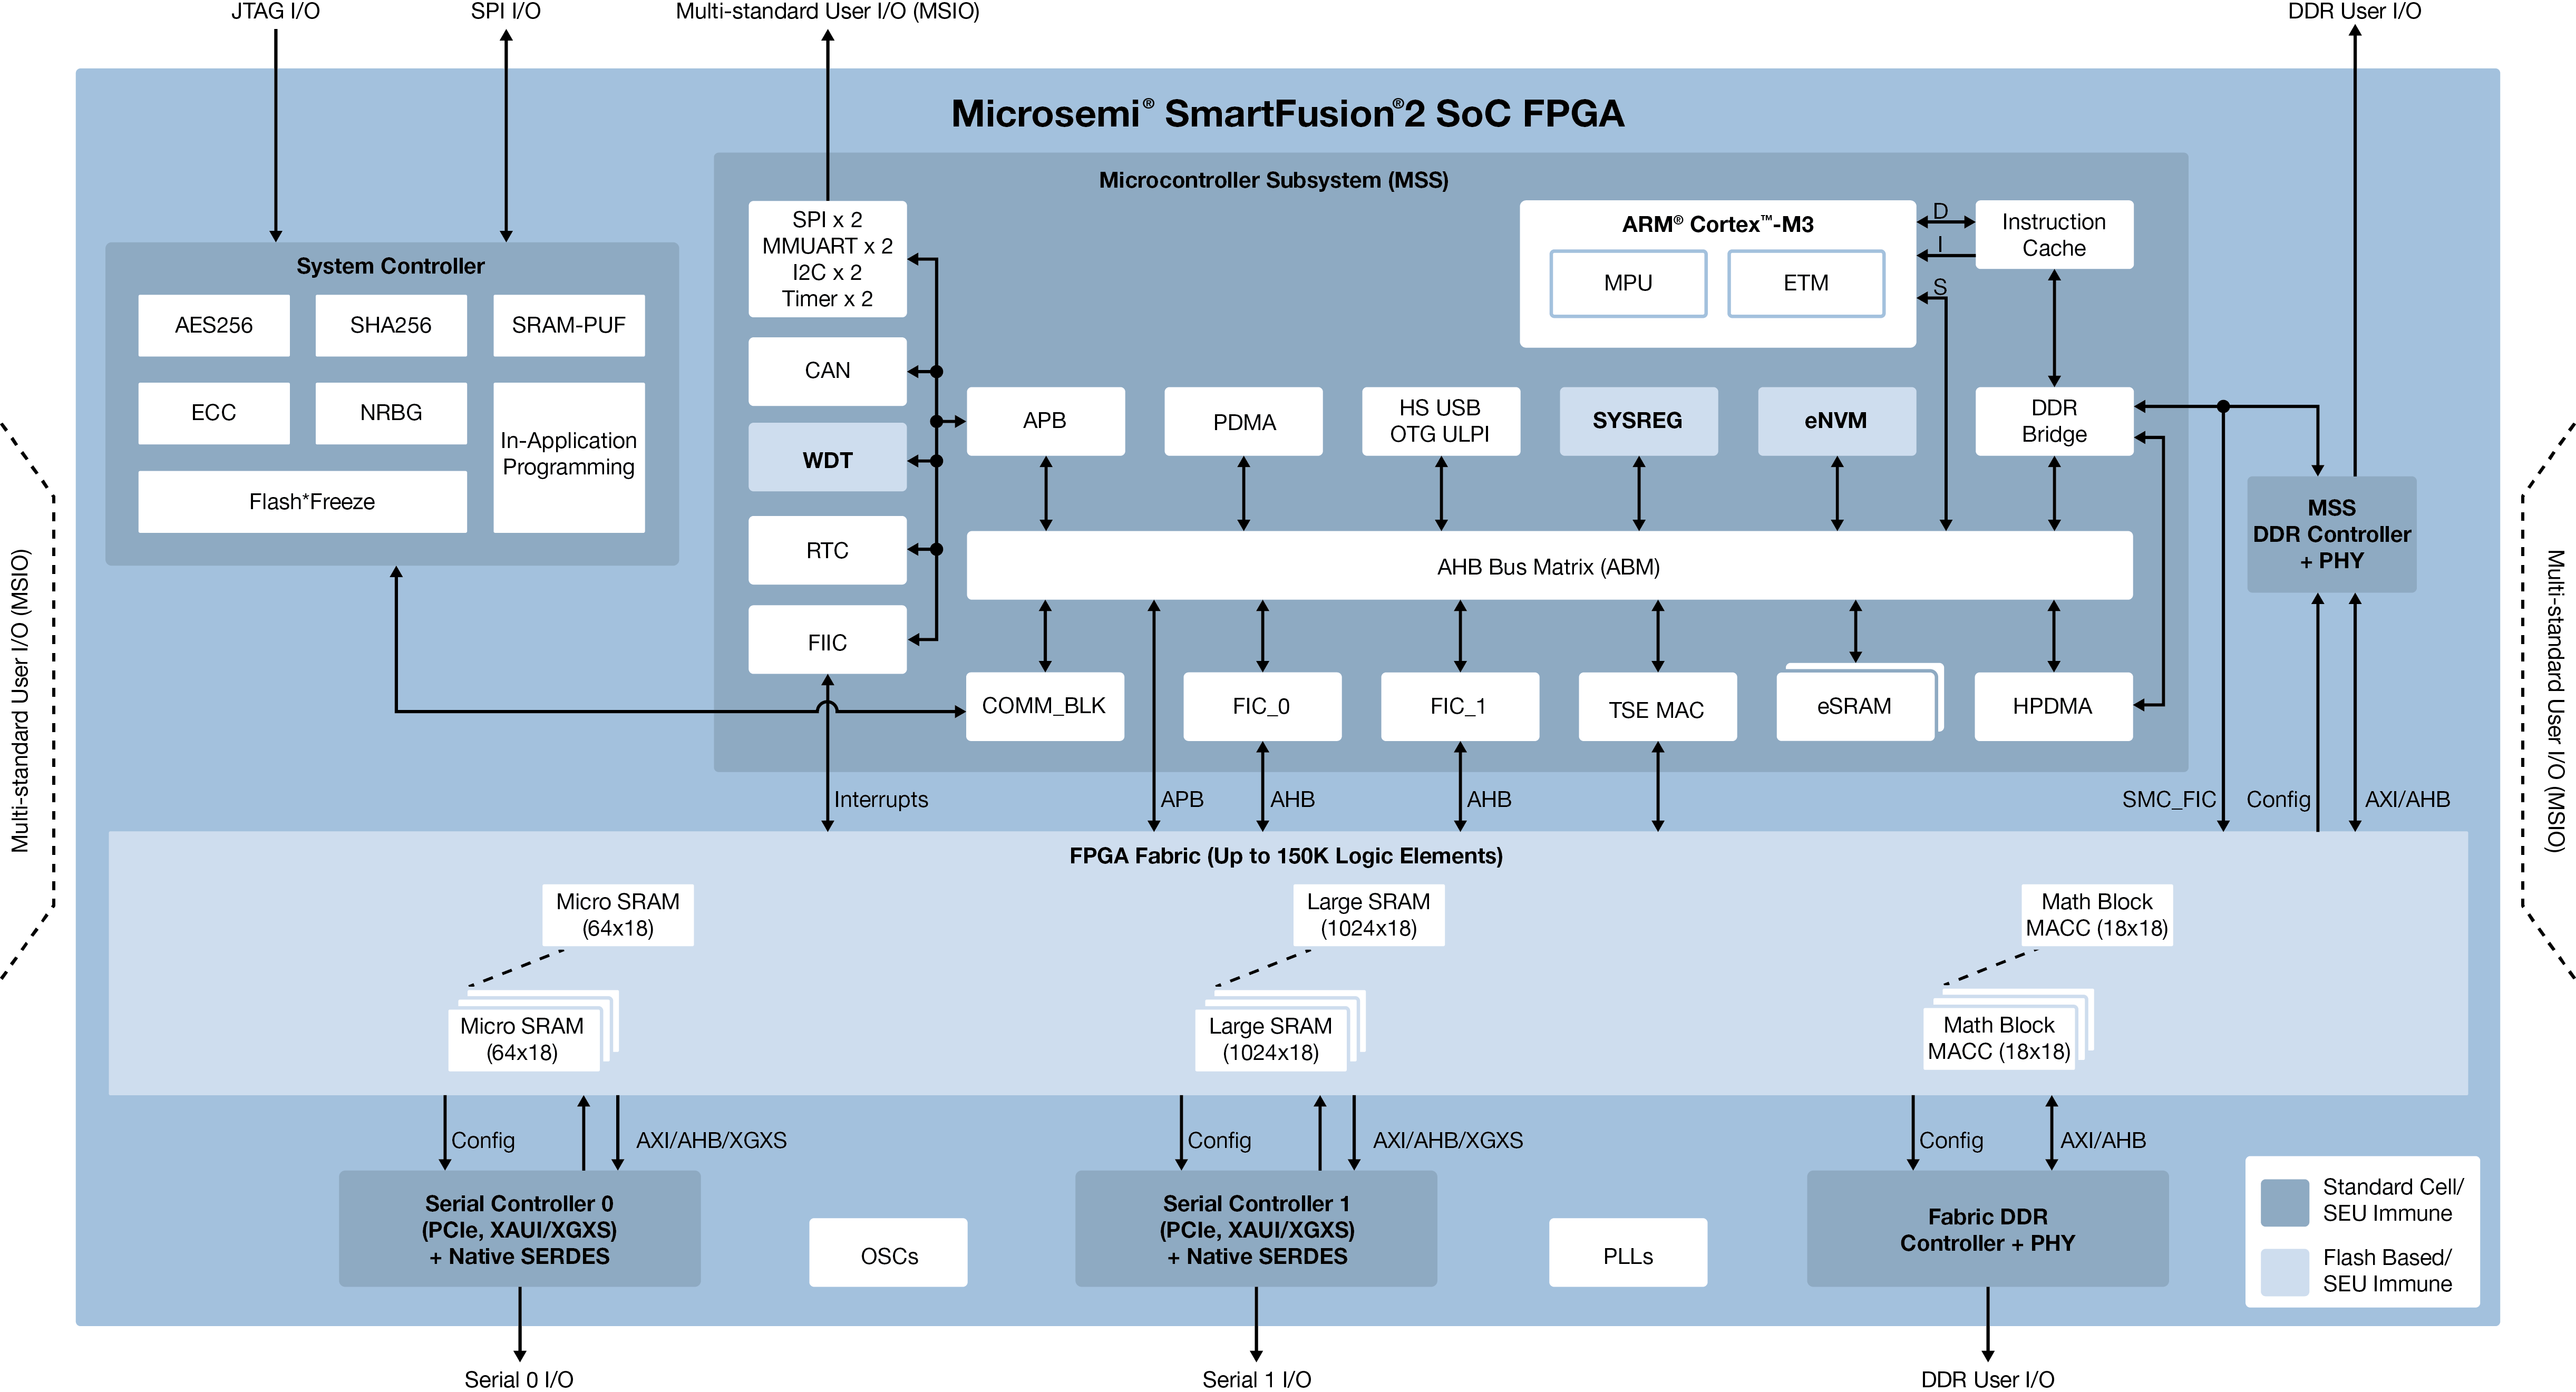
\includegraphics[width=1\textwidth]{./Images/Microsemi_Smartfusion2_BD.png}
    \caption{SmartFusion2 SoC FPGA Components}
    \label{fig:smartfusion2}
\end{figure}

The \ac{AES} system service supports encryption with 128 bit and 256 bit keys, with the following modes: ECB, CBC, OFB and CTR.
It provides a \ac{SHA}-256 hashing service, and a \ac{HMAC} service using the same hashing function.
The KeyTree service provides access to a SHA-256 based key-tree cryptography algorithm. Notably, it can be used to generate a message authentication code from a hash input and key, as a key derivation function with a key and salt as input or in challenge-response protocols.
The \ac{TRNG} service provides a raw entropy source based upon a noisy ring oscillator, measured against a system clock.

The device includes several relevant \ac{ECC} accelerators, with the \ac{NIST} defined P-384 elliptic curve.
It can generate public keys from the corresponding private key, using its scalar point multiplication service, by multiplying the scalar (private key) with the curve's base point. This service also allows the generation of a shared secret with \ac{ECDH}, by multiplying the device's private key with another user's public key.
The device also includes a point addition service, which allows the implementation of the \ac{ECDSA} algorithm for generating digital signatures.

The board provides a SRAM-PUF service to store user supplied or randomly generated keys.  It holds up to 56 key slots with a maximum of 4096 bits each.
It uses the random start-up behaviour of a 2KB \ac{SRAM} block to determine a static secret, unique to each device. There is enough repeatability in the SRAM turn-on behaviour to reconstruct the same secret each time. This secret is used to derive cryptographic keys with 256 bit security strength.
When power is removed, the secret disappears. At present, there is no technology able to detect the start-up behaviour of an SRAM \cite{smartfusionSecurityPractices}. It is determined by atomic-scale manufacturing differences in SRAM transistors.
Each enrolled key generates a key code, required along with the secret to generate the specific key.
The key codes are protected by \ac{AES} encryption and stored in a private section of the eNVM.

The eNVM is a tamper-resistant nonvolatile memory. It has a size of 512KB, with the top 64 pages reserved for keys and passcodes, inaccessible by the user.
It has a limited number of write cycles. For a predicted life span of 20 years, there is a limit of 1000 writes per page of 128 bytes \cite{smartfusionDatasheet}. For a smaller life span of 10 years, it has a limit of 10000 cycles per page.

The side-channel \ac{DPA} is an advanced power analysis technique, to compute values from statistical analysis of multiple cryptographic operations \cite{kocher1999differential}.
Not all services in the SmartFusion2 board are \ac{DPA}-resistant. ECC point multiplication, \ac{NRBG}, SRAM-PUF and KeyTree have strong resistance measures.
On the other hand, AES, SHA-256 and HMAC accelerators have very light countermeasures, and are not considered safe to use repeatedly with the same keys, or in situations where the adversary may be able to choose the ciphertext.
For the non \ac{DPA}-resistant services, there is a danger of key extraction if the same key is used repeatedly.
To extract information with this type of attack, physical access to the device is needed. In this case, the device has tamper detection mechanisms, so its services can be blocked, or the device is completely reset and all sensitive information is deleted.
This feature is called zeroization, and can be run when a tamper attempt is detected or manually by the user.
% To setup this type of attack, physical access to the device is needed with an oscilloscope to measure the voltage \cite{dpaKocher2011}.
% It is advisable for the services to rotate keys in a regular schedule.
% They are all safe of Timing Analysis.
% Tamper detection mechanisms are available so the user can block operations or completely reset the device with zeroization.

%%%%%%%%%%%%%%%%%%%%%%%%%%%%%%%%%%%%%%
\subsection*{Secure boot}

Boot code should be validated before its execution leads to potentially executing untrusted code. This can cause problems such as malware insertion, download of intellectual property or user spying.
Most embedded processors do not validate code before it is executed. The SmartFusion2 \ac{SoC} solves this problem by using a non-volatile memory (eNVM) to store boot code, which is write protected. It authenticates each stage of the boot process, to create a chain-of-trust.
Other systems also implement solutions to secure boot code. Infineon secures the boot process for ARM platforms by incorporating a \ac{TPM} into the platform. The \ac{TPM} operates as a root of trust, to certify the platform's integrity and correct system state. This prevents tampered kernels and fault attacks.
Texas Instruments Sitara processors allow the customer to specify a public key as a root of trust, into the device. This key is used to authenticate other keys, used to authenticate software components.

%%%%%%%%%%%%%%%%%%%%%%%%%%%%%%%%%%%%%%
\section{State of the Art}\label{chap:background:art}

In general, \ac{HSM} have been applied in several contexts, to exploit their cryptographic services, secure storage and physical tamper protections.

Lesjak et al. \cite{iothardware} developed a system to secure remote snapshot acquisition, between the vendor and customers, by attaching a HSM to the products distributed among customers. 
The messages are protected with the authenticated-encryption scheme \ac{AES}-\ac{GCM} and a TLS connection.
The Infineon security controller stores the TLS keys, and protects the data with the authenticated-encryption scheme, using its TRNG and a \ac{DH} based algorithm for key establishment with ECC keys. The controller has protections against side-channel attacks such as \ac{DPA} and physical manipulation.

Seol et al. \cite{trustediaashsm} proposed a system to isolate critical operations and sensitive data from cloud administrators, by implementing a \ac{HSM} next to a virtual machine.

Wolf et al. \cite{wolf2011design} implemented a HSM on a 663€ Xilinx Virtex-5 FPGA to secure network communications in vehicles. The authors implemented several cryptographic algorithms on the FPGA, e.g., AES-128 bit and ECC point-multiplication with a 256 bit curve. The board was connected to a microcontroller running linux, with additional algorithms available from a cryptographic library.

An IBM 4764 PCI-X cryptographic coprocessor has been used to store and manage symmetric keys, which encrypt biomedical data \cite{canim2011biomedical}. The symmetric keys, which encrypt the database, are transferred to the device using public-key cryptography. All database queries are performed by the coprocessor, since only it has the keys. The system uses AES with 128 bit encryption. Notably, the device has physical measures which ensure the keys are not leaked and the data is erased upon any attack.

Wherry \cite{wherry2003secure} recognizes the need for a HSM PKIs to protect the cryptographic keys.
Lorch et al. \cite{lorch2004hardware} uses an IBM 4758 cryptographic coprocessor to protect keys in a secure online repository for PKIs. The authors were able to store more than 800 2048-bit RSA key pairs on the device's secure storage. The PKI system interfaces with the HSM using a PKCS\#11 interface. Keys are generated in the coprocessor and the private key is never extracted. The RSA implementation is used to sign certificates, while the public key can be extracted to the application. A PIN is necessary to access the coprocessor.

Several protocols and HSM applications have also been proposed.
Rössler et al. \cite{rossler2005voting} applied a HSM to an e-voting electronic ballot box. The HSM is used for decrypting and verifying the signature of cast votes.
The votes decryption is done solely inside the electronic ballot box during the counting process.
Voters sign their ballot using a smart card, e.g., their citizen card.
Only the HSM is capable of counting votes, using its private key.
The author recommends 1024 bit RSA or 160 bit ECC keys for an actual implementation.

Additionally, authors have proposed using a HSM to secure web services by providing secure storage for keys and cryptography algorithms in the TLS protocol, but also for providing a complete security service, not just an algorithm implementation \cite{baldwin2003hardware}, \cite{mont2003secure}.

% include openHSM?
Martina et al. \cite{openhsm} presents OpenHSM, an open cryptographic protocol to manage private keys in an application embedded in a HSM.
The protocol was implemented with a customized FreeBSD system. The authors introduced administrator and operator groups to manage
private keys inside the HSM. The hardware was projected to be tamper proof using a Security Unit to manage all sensors and protection mechanisms.
The OpenSSL library and SQLite database were used to provide smart card support, data storage, secret sharing and X509v3 certificates.

% -------------------------
Several HSMs on the market have been studied.
Kehret et al. \cite{tlsintegration} studied two devices. VaultIC460, a secure microcontroller manufactured by Inside Secure with a RISC CPU. It includes a varied offering of cryptographic algorithms, such as, AES encryption, public-key cryptography with RSA and ECC, MAC, SHA, SSL support, as well as a random number generator. Additionally it includes several authentication mechanisms for users, to secure the connection between the application and device.
It includes 112 KB of tamper resistant memory for key storage.
ATECC508A from Microsemi is a small security controller with the asymmetric key algorithms: ECDSA and ECDH, along with SHA, a TRNG and storage of up to sixteen 256 bit keys.
This type of controllers, in general, are not suitable for this work. They are very limited, with no symmetric key algorithms, preventing encryption of large amounts of data. They are designed to be added to Internet of Things devices.

The survey \cite{ivarsson2010review} studies the features of four \ac{HSM} on the market, Keyper v2 by AEP, nShield Connect 6000 by Thales, Safenet Luna and Utimaco CryptoServer.
All devices support authentication using smartcards, password or a PIN. The AEP and Utimaco also have additional smartcard integration, for backing up the device's internal keys.
All devices have tamper resistant storage, a \ac{TRNG}, as well as a varied range of supported cryptographic services. Several AES encryption modes for both 128 and 256 bit keys, SHA, HMAC and public-key cryptography with RSA.
ECDSA and ECDH are supported by the devices from Safenet and Utimaco.
All devices provide a PKCS\#11 interface implementation for all cryptography services. The provided API can be used to build an application adapted to each user's requirements. The PKCS\#11 implementation does not output any unencrypted sensitive information, such as keys.

HSMs on the market go from 650€ up to \$39,000 \cite{HSMpriceArticles}, \cite{HSMPresentationPrices}.
One of the smallest and cheapest devices, the YubiHSM 2 by Yubico \cite{YubiHSM2}, is a \ac{USB} sized device for 650€. It supports several SHA algorithms, RSA, the asymmetric key ECC algorithms: ECDSA and ECDH, with multiple curves, a \ac{TRNG} and the \ac{AES}-\ac{CCM} authenticated encryption algorithm.
It provides a PKCS\#11 implementation, 128KB of tamper resistant storage for keys, and an authenticated and encrypted connection, between the PKCS\#11 API calls and the device.
For comparison, a M2S090TS SmartFusion2 evaluation kit is priced at 384 € \cite{smartfusionPrice}.
